\chapterbegin{Concentrador}
\label{chp:concentrador}
\minitoc

\sectionx{Introducci�n}
\sectionx{Diagrama de bloques y modelo de la interfaz}
\begin{figure}[h]
	\centering
	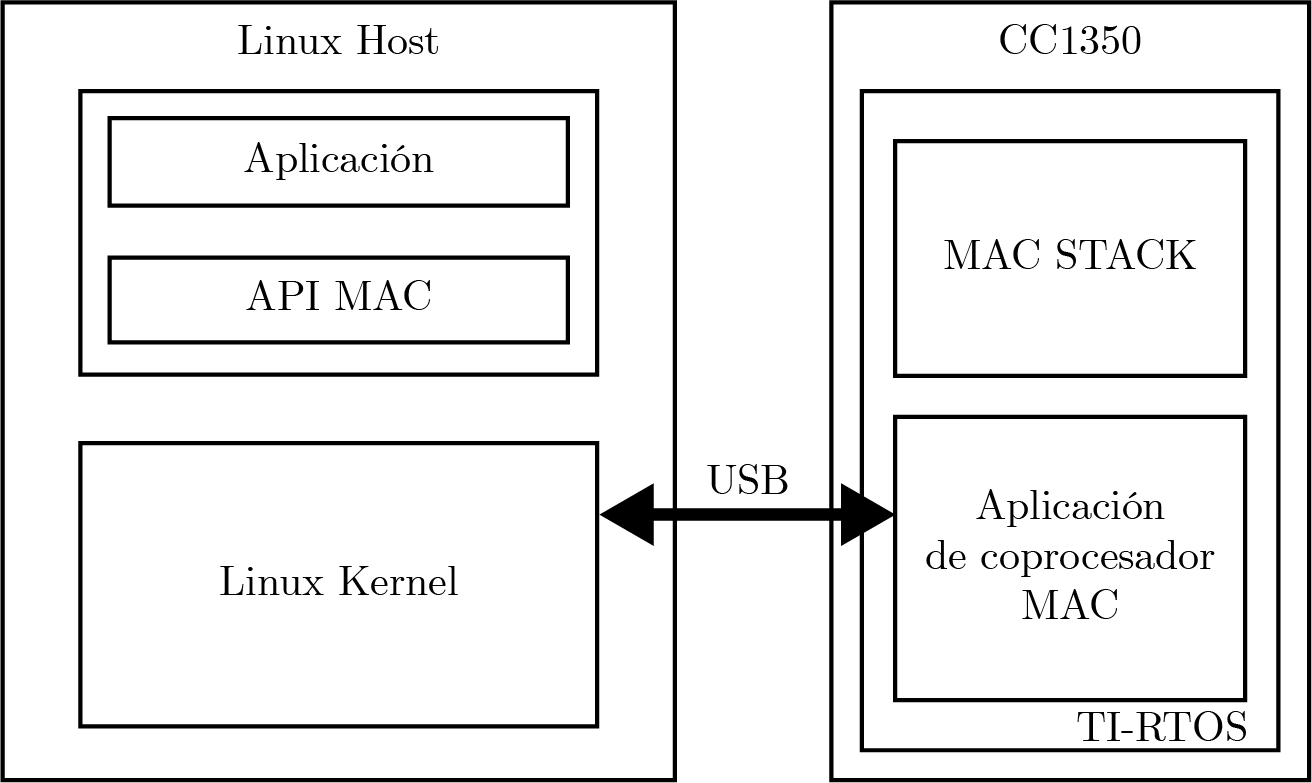
\includegraphics[width=0.8\textwidth]{graphs/concentradorBlockDiagram.png}
	\caption{Arquitectura de software a alto nivel de las aplicaciones TI 15.4-Stack 2.1.0 Linux\R}
	\label{fig:concentradorBlockDiagram}
\end{figure}

Esta secci�n describe la arquitectura de alto nivel basada en coprocesador, los componentes software, y  la arquitectura general del sistema (ve�se figura \ref{fig:concentradorBlockDiagram}). El coprocesador es una entidad que implementa el est�ndar MAC IEEE 802.15.4e/g en un chip dedicado y provee una interfaz serie por la que un procesador externo controla y procesa las operaciones del coprocesador. \\

El coprocesador se centra en una arquitectura escalable con una divisi�n perfecta donde el procesador ejecuta las capas sobre el IEEE 802.15.4e/g MAC/PHY.\\

En esta aplicaci�n, el programa se ejecuta en una plataforma basada en Linux. Aunque los componentes de alto nivel , pueden ser conceptualmente aplicados a otras plataformas no basadas en Linux. Los componentes desarrollados ser�n descritos m�s adelante.\\

La interfaz entre el procesador y el coprocesador est�n definidas como capas l�gicas que est�n separadas en esta arquitectura: una capa f�sica (por ejemplo, USB o UART), una capa l�gica de enlace, y la capa de presentaci�n.\\

Componentes software:

\begin{description}
	\item[Aplicaci�n del coprocesador: ] Es el programa ejecutandose en el dispositivo CC1350. Esta aplicaci�n implementa una capa 802.15.4e/g MAC/PHY y proporciona una comunicaci�n serie.
	\item[Kernel Linux]: El kernel Linux provee los controladores para la interfaz serie que est� disponible en un puerto f�sico (por ejemplo, USB).
	\item[Aplicaci�n TI 15.4-Stack: ] Este m�dulo implementa la aplicaci�n usando el protocolo 802.15.4e/g y la estructura del modelo \ac{MT}.
\end{description}

\sectionx{Descripci�n del SDK}
\begin{figure}{h}
	\begin{center}
		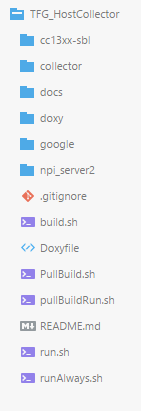
\includegraphics[width=0.5\textwidth]{graphs/fig-oob-dir}
	\end{center}
	\caption{Estructura del directorio TI 15.4-Stack 2.1.0 Linux\R }
	\label{fig:fig-oob-dir}
\end{figure}

La figura \ref{fig:fig-oob-dir} muestra la estructura del directorio de instalaci�n del TI 15.4-Stack 2.1.0. A continuaci�n se explica una descripci�n de alto nivel de cada carpeta:

\begin{description}
	\item[components: ] Contiene las siguientes librer�as:
	\begin{description}
		\item[common: ] Rutinas para caracter�sticas del sistema operativo, como lectura y escritura de ficheros.
		\item[nv: ]  Simula una memoria no vol�til, como la usada en sistemas empotrados.
		\item[api: ] Interfaz de mensajes API MAC y MT
	\end{description}
	\item[docs: ] Documentos como la gu�a de desarrollo y la gu�a de comandos MAC para el coprocesador.
	\item[example: ] Aplicaci�n de ejemplo
	\begin{description}
		\item[cc13xx-sbl: ] Herramientas para la actualizaci�n para los dispositivos CC13x0.
		\item[collector: ]  Aplicaci�n de ejemplo que demuestra como iniciar una red, permitir la conexi�n de dispositivos y recoger datos desde dispositivos remotos.
		\item[gateway: ] Una aplicaci�n basada en Node.js\TM que crea un servidor local y muestra la informaci�n de la red y los datos de los nodos.
		\item[npi\_server2: ] Interfaz socket para comunicarse con el coprocesador.
		\item[google: ] Contiene un makefile para descargar e instalar el compilador de \textit{Google protocol buffer}.
	\end{description}
	\item[firmware] Precompilados ficheros .hex para el coprocesador.
	\item[prebuilt] Compilaci�n para ejecutar la aplicaci�n de ejemplo en una BeagleBone Black.
	\item[scripts] Contiene fragmentos de ficheros makefile usados para compilar la aplicaci�n de ejemplo.
\end{description}

\sectionx{Aplicaci�n}




\chapterend{}